\chapter{Implementacija i korisničko sučelje}


\section{Korištene tehnologije i alati}

Komunikacija u timu odrađena je pomoću aplikacija \underbar{Whatsapp}\textsuperscript{1} i \underbar{Discord}\textsuperscript{2}. Za potrebe izrade dijagrama korišten je alat \underbar{Astah UML}\textsuperscript{3}. Kao sustav za praćenje verzija i upravljanja kodom korišten je \underbar{Git}\textsuperscript{4}, a kao zajednički repozitorij korišten je \underbar{GitHub}\textsuperscript{5}.
Kao razvojno okruženje za potrebe frontend developmenta korišten je \underbar{Visual studio code}\textsuperscript{6} tvrtke Microsoft, a za potrebe izrade backend dijela korišten je \underbar{IntelliJ}\textsuperscript{7} tvrtke JetBrains. \newline
Za izradu frontend dijela korišten je \underbar{React}\textsuperscript{8}, kojeg je napravila i usavršila tvrtka Meta, \underbar{Chakra UI}\textsuperscript{9} kao alternativu css-u, a za izradu backend dijela aplikacije korišten je okvir \underbar{SpringBoot}\textsuperscript{10}.
React je jedan od najpopularnijih okvira za izradu frontend dijela web aplikacije te se lako mogu pronaći potrebne informacije o njegovom korištenju. React se vrlo dobro uklapa sa SpringBootom koji također ima vrlo široku primjenu i veliku zajednicu developera.
Baza podataka je napravljena koristeći \underbar{PostgreSQL}\textsuperscript{11} i nalazi se na poslužitelju.
Za testiranje aplikacije korišteni su \underbar{Postman}\textsuperscript{12} i \underbar{Selenium}\textsuperscript{13}.\\

\footnotesize \begin{enumerate}
	\itemsep0em
	\item \url{https://www.whatsapp.com/}
	\item \url{https://discord.com/}
	\item \url{https://astah.net/}
	\item \url{https://git-scm.com/}
	\item \url{https://github.com/}
	\item \url{https://code.visualstudio.com/}
	\item \url{https://www.jetbrains.com/idea/}
	\item \url{https://react.dev/}
	\item \url{https://chakra-ui.com/}
	\item \url{https://spring.io/projects/spring-boot/}
	\item \url{https://www.postgresql.org/}
	\item \url{https://www.postman.com/}
	\item \url{https://www.selenium.dev/}
\end{enumerate}

\eject 


\section{Ispitivanje programskog rješenja}


\subsection{Ispitivanje komponenti}
\textnormal{Ispitivanje komponenti koristi se za verificiranje rada programskih dijelova koje je moguće zasebno ispitati u izolaciji. Najčešće se ispitiju pojedinačne funkcije ili metode unutar raznih objekata.}\\

\noindent \textbf{1. ispitni slučaj: Ispitivanje metode za validaciju emaila slanjem neispravnog oblika maila}\\
U ovom ispitivanju testiramo rad metode za provjeru je li email dobrog oblika. Testiramo na način da pošaljemo email koji nije validan. Test hvata iznimku te ako je test prošao, to znači da se dogodila iznimka i email nije validan. Šaljemo mail "email00". U svrhu testa metoda je pretvorena u public metodu, a u kodu je ostavljena kao private. \\
\textbf{Kôd testa:}
\begin{figure}[H]
	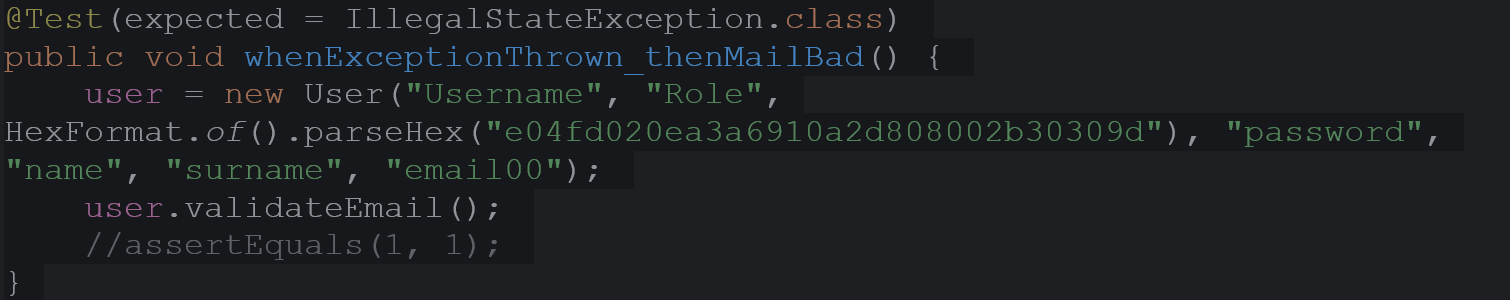
\includegraphics[scale=0.5]{slike/kodTesta1.PNG} %veličina slike u odnosu na originalnu datoteku i pozicija slike
	\centering
\end{figure}
\noindent \textbf{Rezultat:}
\begin{figure}[H]
	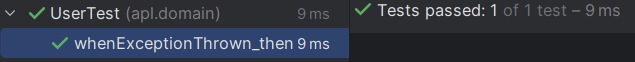
\includegraphics[scale=0.7]{slike/test1.PNG} %veličina slike u odnosu na originalnu datoteku i pozicija slike
	\centering
\end{figure}
\noindent Zadan je neispravan oblik emaila, test je prošao što je u ovom slučaju i očekivano. \\

\noindent \textbf{2. ispitni slučaj: Ispitivanje metode za validaciju emaila slanjem ispravnog oblika maila}\\
U ovom ispitivanju testiramo rad metode za provjeru je li email dobrog oblika. Testiramo na način da pošaljemo email koji je validan. Test hvata iznimku te ako je test prošao, to znači da se dogodila iznimka i email nije validan. Ako se nije dogodila iznimka, test nije prošao i email je validan. Šaljemo mail "email@mail.com". U svrhu testa metoda je pretvorena u public metodu, a u kodu je ostavljena kao private. \\
\textbf{Kôd testa:}
\begin{figure}[H]
	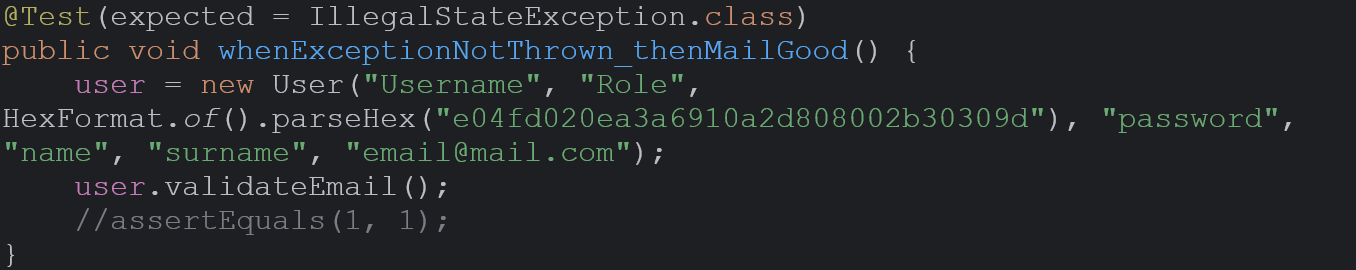
\includegraphics[scale=0.5]{slike/kodTesta2.PNG} %veličina slike u odnosu na originalnu datoteku i pozicija slike
	\centering
\end{figure}
\noindent \textbf{Rezultat:}
\begin{figure}[H]
	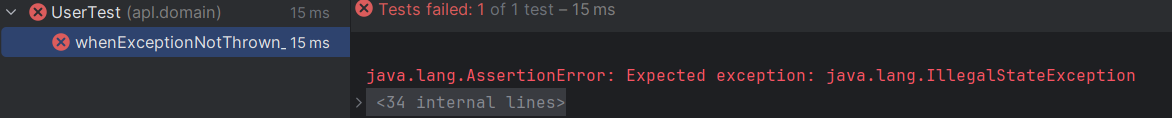
\includegraphics[scale=0.6]{slike/test2.PNG} %veličina slike u odnosu na originalnu datoteku i pozicija slike
	\centering
\end{figure}
\noindent Zadan je ispravan oblik emaila i test nije prošao što je očekivan rezultat. \\

\noindent \textbf{3. ispitni slučaj: ispitivanje metode za validaciju korisničkog imena(username) unoseći ispravan username}\\
U ovom ispitivanju testiramo rad metode za provjeru je li username dobrog oblika. Testiramo na način da pošaljemo username koji je validan. Test hvata iznimku te ako je test prošao, to znači da se dogodila iznimka i username nije validan. Ako se nije dogodila iznimka, test nije prošao i username je validan. Testiramo username "12345". U svrhu testa metoda je pretvorena u public metodu, a u kodu je ostavljena kao private. \\
\textbf{Kôd testa:}
\begin{figure}[H]
	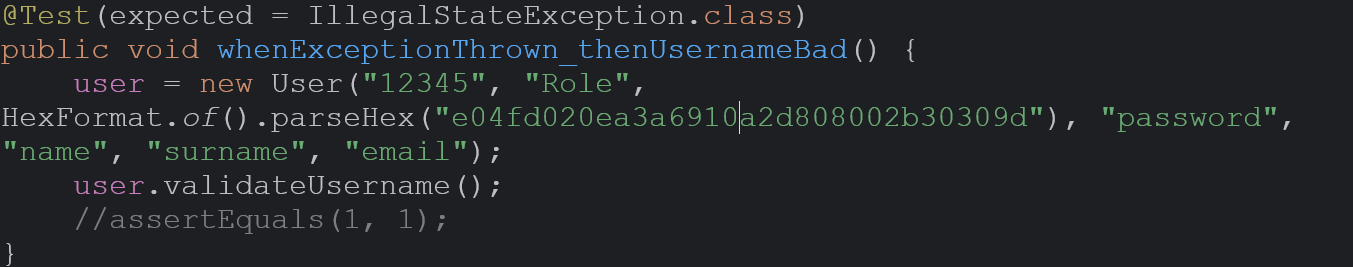
\includegraphics[scale=0.5]{slike/kodTesta3.PNG} %veličina slike u odnosu na originalnu datoteku i pozicija slike
	\centering
\end{figure}
\noindent \textbf{Rezultat:}
\begin{figure}[H]
	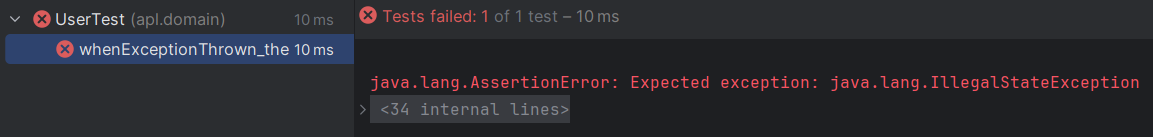
\includegraphics[scale=0.6]{slike/test3.PNG} %veličina slike u odnosu na originalnu datoteku i pozicija slike
	\centering
\end{figure}
\noindent Zadan je ispravan oblik usernamea i test nije prošao što je očekivan rezultat. \\

\noindent \textbf{4. ispitni slučaj: ispitivanje metode za validaciju korisničkog imena(username) unoseći naizgled ispravan username}\\
U ovom ispitivanju testiramo rad metode za provjeru je li username dobrog oblika. Testiramo na način da pošaljemo username koji je naizgled validan. Test hvata iznimku te ako je test prošao, to znači da se dogodila iznimka i username nije validan. Ako se nije dogodila iznimka, test nije prošao i username je validan. Testiramo username "User1\#\#". U svrhu testa metoda je pretvorena u public metodu, a u kodu je ostavljena kao private. \\
\textbf{Kôd testa:}
\begin{figure}[H]
	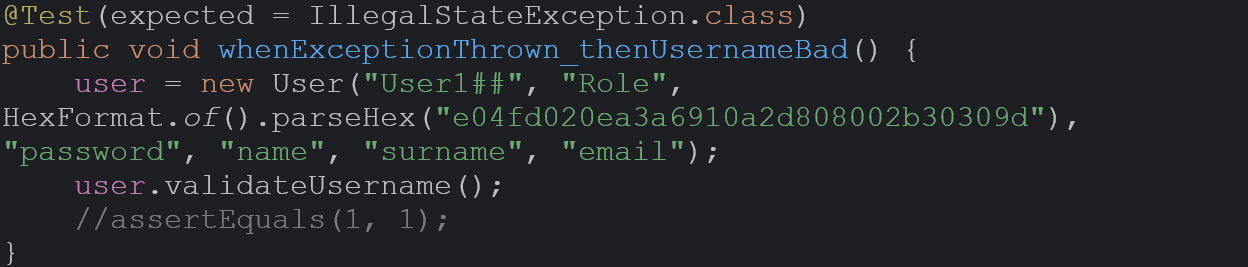
\includegraphics[scale=0.5]{slike/kodTesta4.PNG} %veličina slike u odnosu na originalnu datoteku i pozicija slike
	\centering
\end{figure}
\noindent \textbf{Rezultat:}
\begin{figure}[H]
	
\includegraphics[scale=0.6]{slike/test4.PNG} %veličina slike u odnosu na originalnu datoteku i pozicija slike
	\centering
\end{figure}
\noindent Zadan je neispravan oblik usernamea i test je prošao što je očekivan rezultat. \\

\noindent \textbf{5. ispitni slučaj: ispitivanje metode za provjeru vremena unutar intervala}\\
U ovom ispitivanju testiramo rad metode za provjeru je li određeni datum unutar dva zadana intervala. Test će proći ako je zadani datum unutar intervala. Testirat ćemo rubni slučaj koji ispituje nalazi li se datum 13.1.2024. unutar intervala 13.1.2024. – 24.1.2024. \\
\textbf{Kôd testa:}
\begin{figure}[H]
	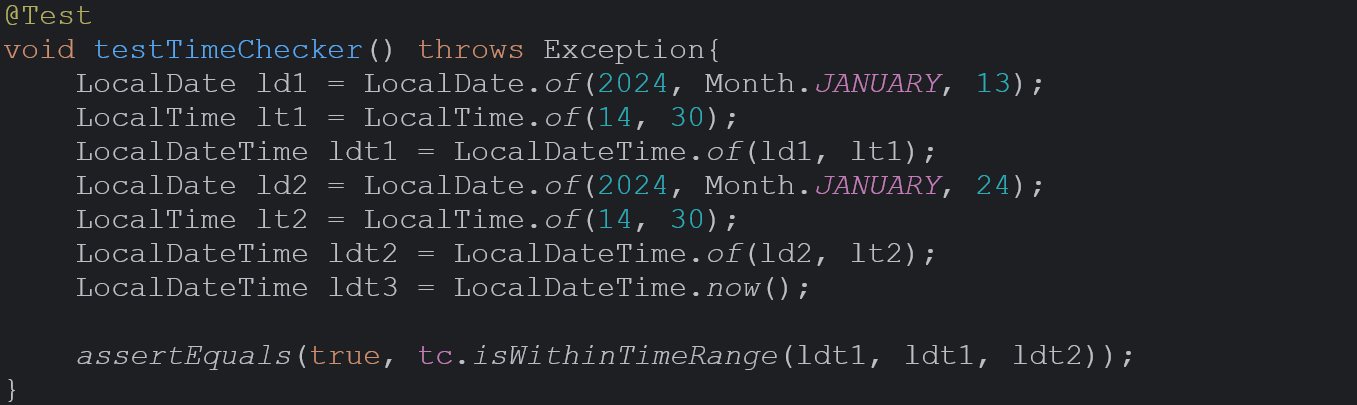
\includegraphics[scale=0.5]{slike/kodTesta5.PNG} %veličina slike u odnosu na originalnu datoteku i pozicija slike
	\centering
\end{figure}
\noindent \textbf{Rezultat:}
\begin{figure}[H]
	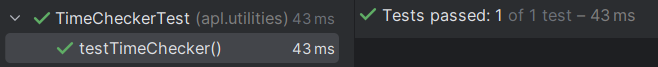
\includegraphics[scale=0.6]{slike/test5.PNG} %veličina slike u odnosu na originalnu datoteku i pozicija slike
	\centering
\end{figure}
\noindent Zadan je datum koji je na granici intervala te je test prošao što je očekivan rezultat. \\

\noindent \textbf{6. ispitni slučaj: ispitivanje metode za provjeru vremena unutar intervala}\\
U ovom ispitivanju testiramo rad metode za provjeru je li određeni datum unutar dva zadana intervala. Test će proći ako je zadani datum unutar intervala. Testirat ćemo rubni slučaj koji ispituje nalazi li se datum 13.1.2024. unutar intervala null – null. \\
\textbf{Kôd testa:}
\begin{figure}[H]
	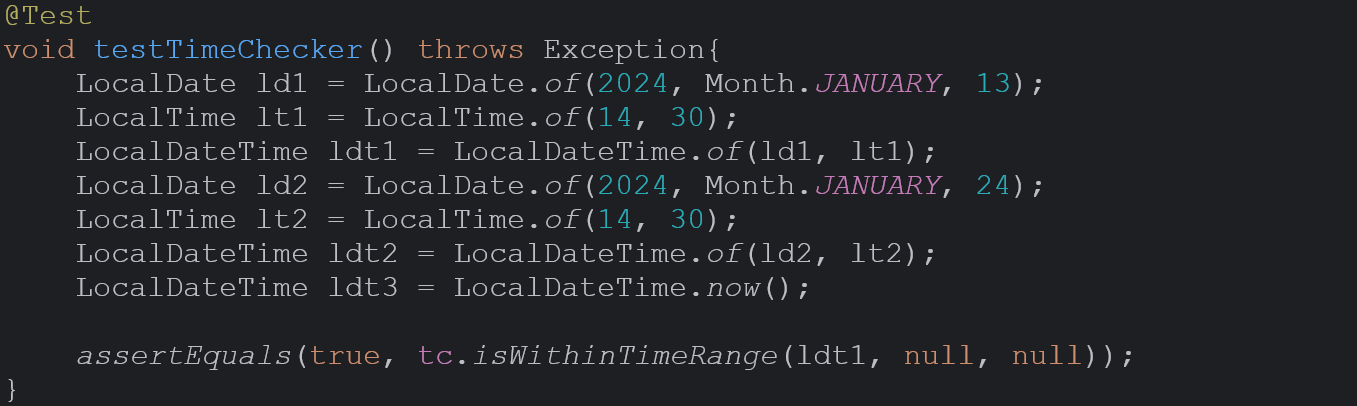
\includegraphics[scale=0.5]{slike/kodTesta6.PNG} %veličina slike u odnosu na originalnu datoteku i pozicija slike
	\centering
\end{figure}
\noindent \textbf{Rezultat:}
\begin{figure}[H]
	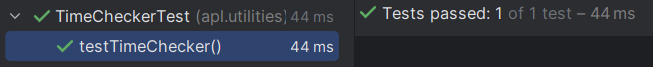
\includegraphics[scale=0.6]{slike/test6.PNG} %veličina slike u odnosu na originalnu datoteku i pozicija slike
	\centering
\end{figure}
\noindent Zadani su intervali null i null. Test je prošao što je očekivan rezultat jer se svaki datum nalazi unutar nepostojećeg intervala.


\subsection{Ispitivanje sustava}

\noindent Proces ispitivanja završene i potpuno integrirane inačice namijenjene distribuciji korisniku. Ispitivanje sustava povećava razinu povjerenja prije nego što proizvod krene na ispitivanje prihvatljivosti, a osnovni cilj je provjera podudarnosti sustava s funkcijskim zahtjevima. \\

\noindent \textbf{1. ispitni slučaj: Ispitivanje unosa pogrešne lozinke prilikom prijave}\\
U ovom ispitivanju testiramo otpornost sustava na unos pogrešne lozinke prilikom korisnikove prijave. Očekuje se da sustav neće dopustiti prijavu te da će ispisati odgovarajuću poruku. \\
\textbf{Test:}
\begin{figure}[H]
	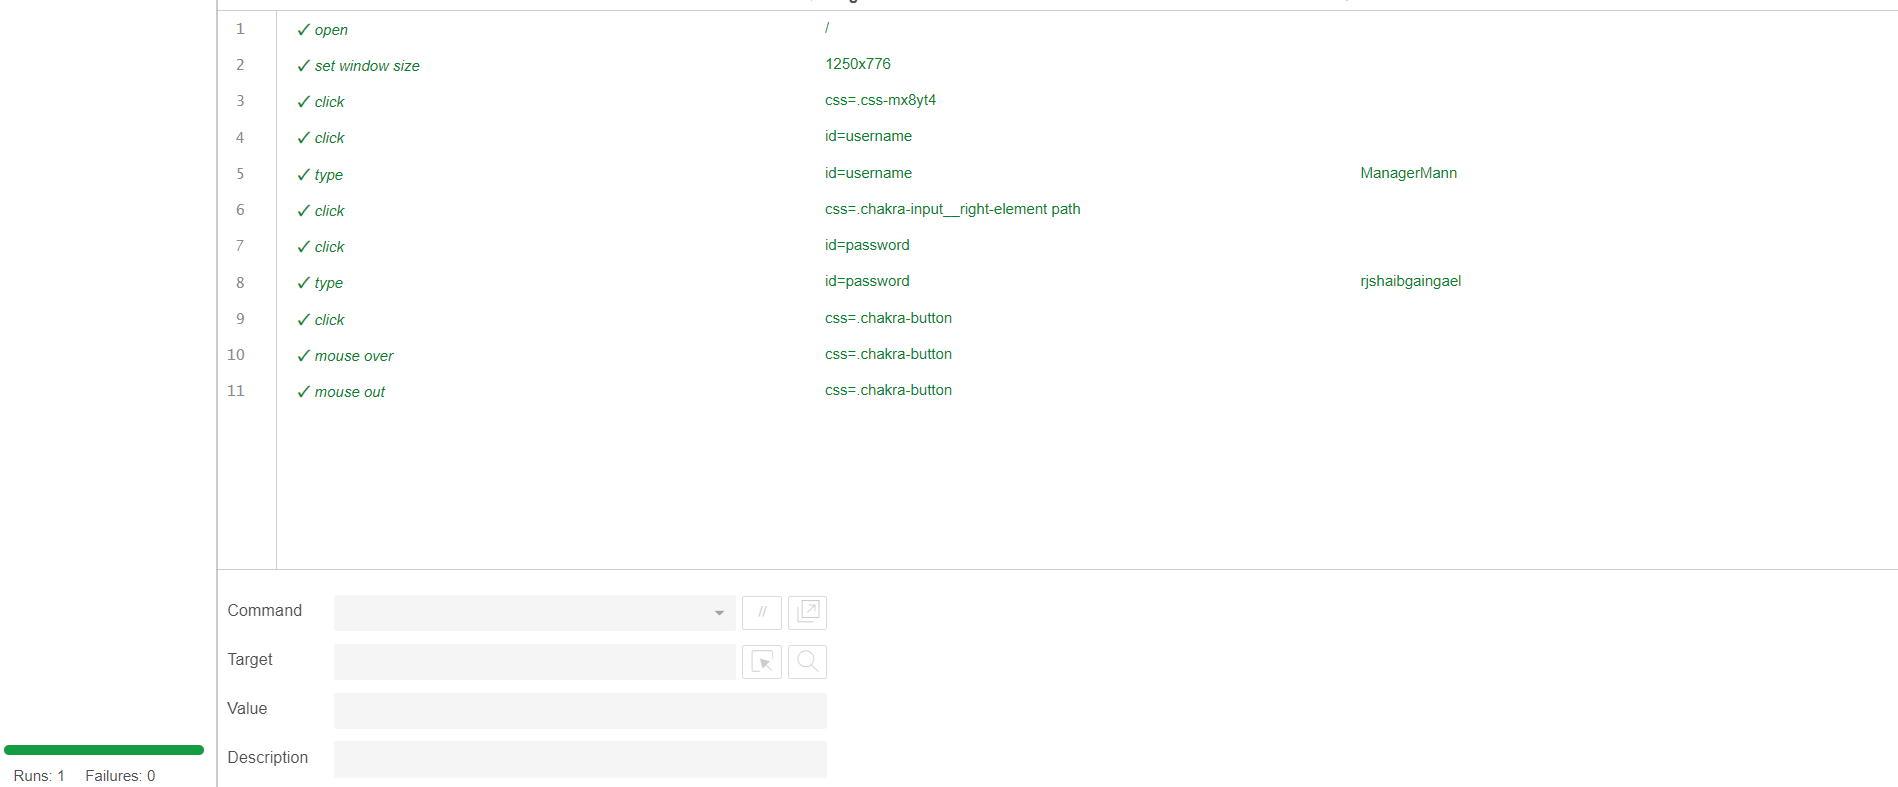
\includegraphics[scale=0.4]{slike/selTest1.PNG} %veličina slike u odnosu na originalnu datoteku i pozicija slike
	\centering
\end{figure}
\noindent \textbf{Rezultat:}
\begin{figure}[H]
	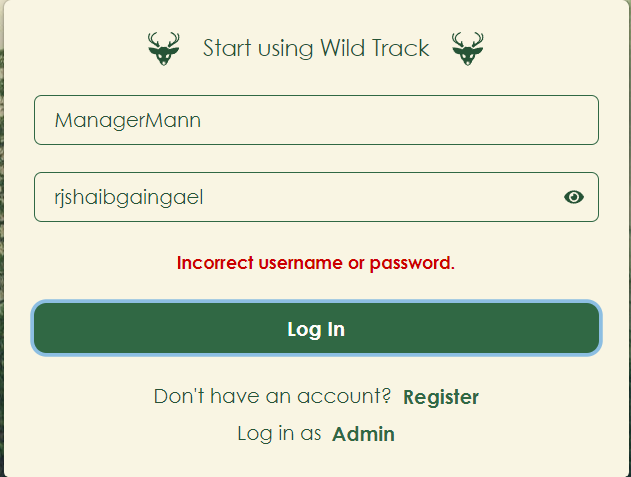
\includegraphics[scale=0.6]{slike/selTestRes1.PNG} %veličina slike u odnosu na originalnu datoteku i pozicija slike
	\centering
\end{figure}
\noindent Aplikacija ne dopušta prijavu i ispisuje se odgovarajuća poruka korisniku. \\

\noindent \textbf{2. ispitni slučaj: Ispitivanje pregleda zahtjeva kod voditelja}\\
U ovom ispitivanju testiramo kako sustav odgovara ako pokušamo pregledati zahtjeve tragača. Voditelj nije primio niti jedan zahtjev od strane tragača pa očekujemo da sustav ne daje krive informacije. \\
\textbf{Test:}
\begin{figure}[H]
	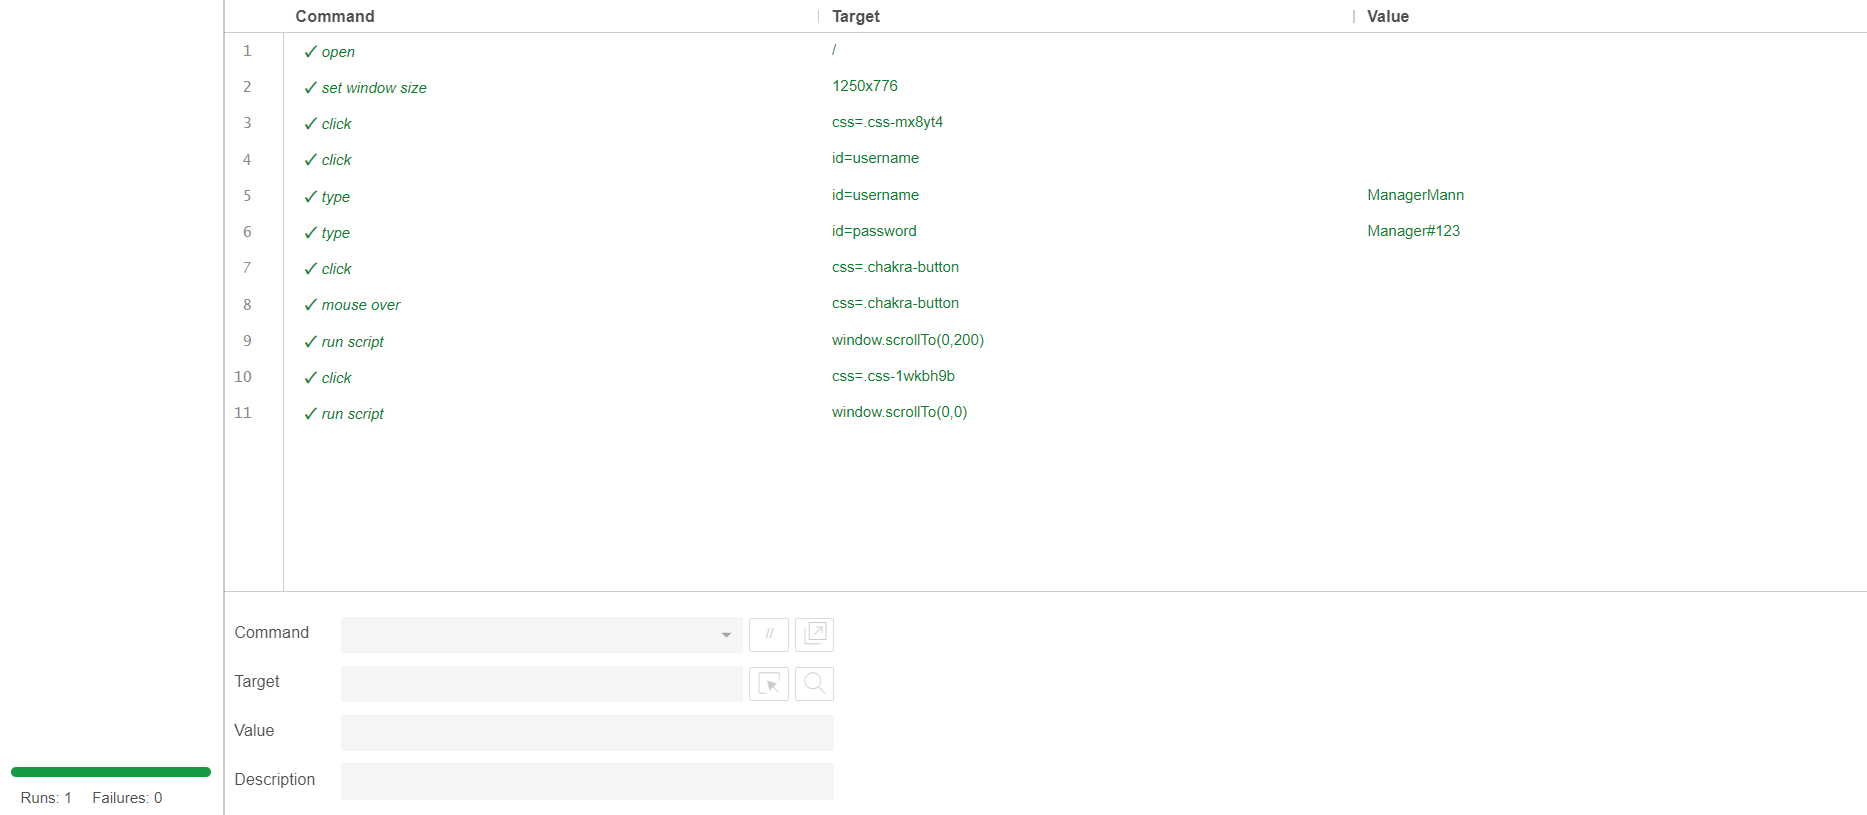
\includegraphics[scale=0.4]{slike/test2sel.PNG} %veličina slike u odnosu na originalnu datoteku i pozicija slike
	\centering
\end{figure}
\noindent \textbf{Rezultat:}
\begin{figure}[H]
	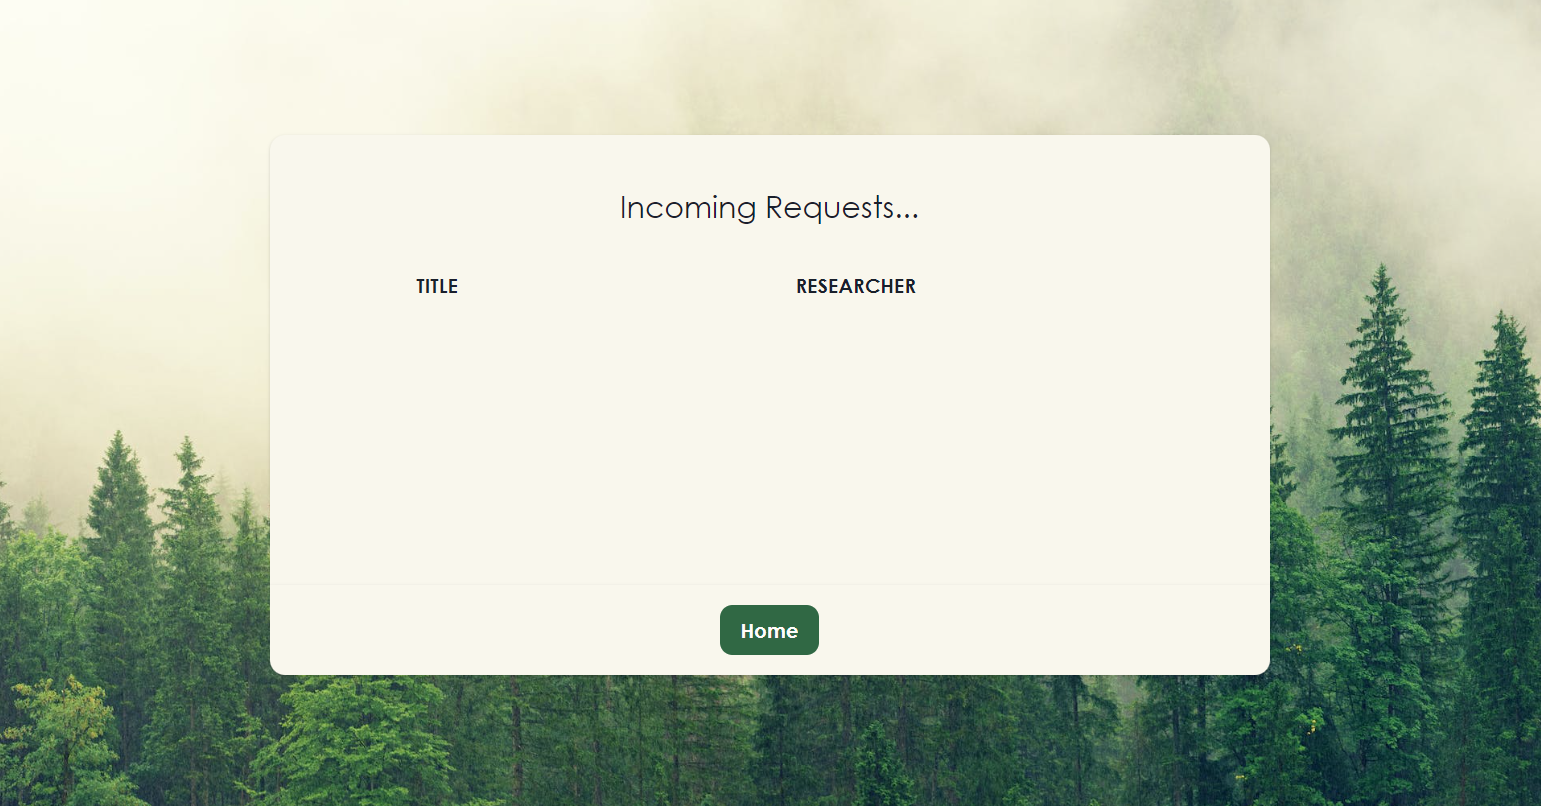
\includegraphics[scale=0.5]{slike/test2selrez.PNG} %veličina slike u odnosu na originalnu datoteku i pozicija slike
	\centering
\end{figure}
\noindent Aplikacija ne ispisuje nikakav višak informacija i prikazuje se prazna stranica jer nema zahtjeva. \\

\noindent \textbf{3. ispitni slučaj: Ispitivanje potvrde od strane admina}\\
U ovom ispitivanju testiramo potvrđivanje korisnika od strane administratora. Očekujemo da administrator, nakon prijave korisnika, može potvrditi korisnika. \\
\textbf{Test:}
\begin{figure}[H]
	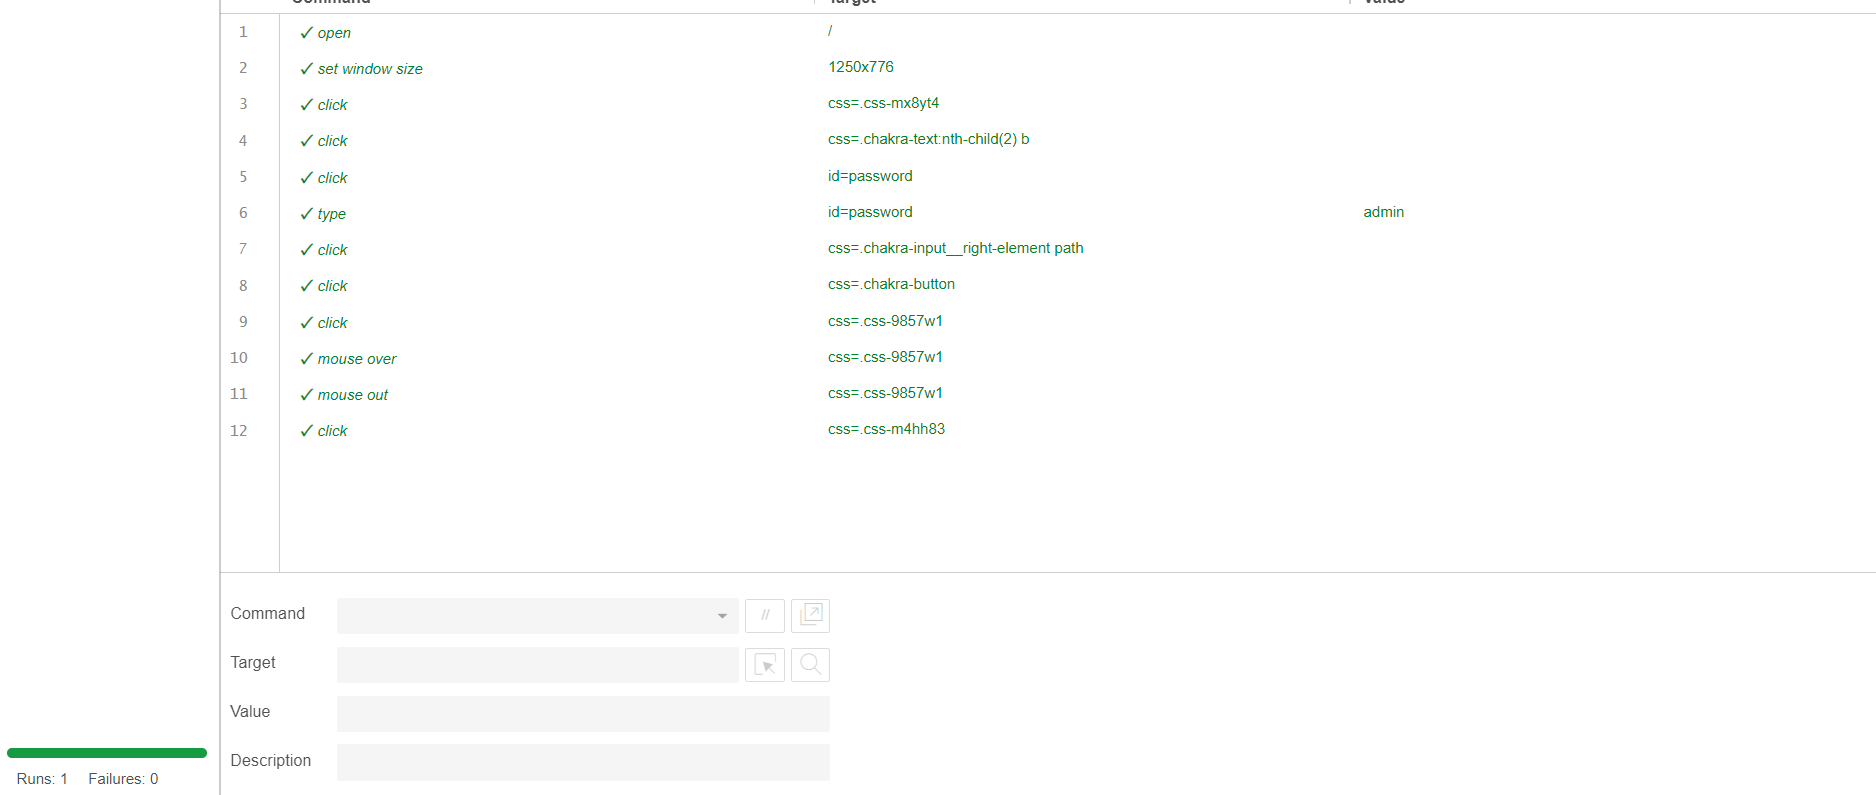
\includegraphics[scale=0.4]{slike/test3sel.PNG} %veličina slike u odnosu na originalnu datoteku i pozicija slike
	\centering
\end{figure}
\noindent \textbf{Rezultat:}
\begin{figure}[H]
	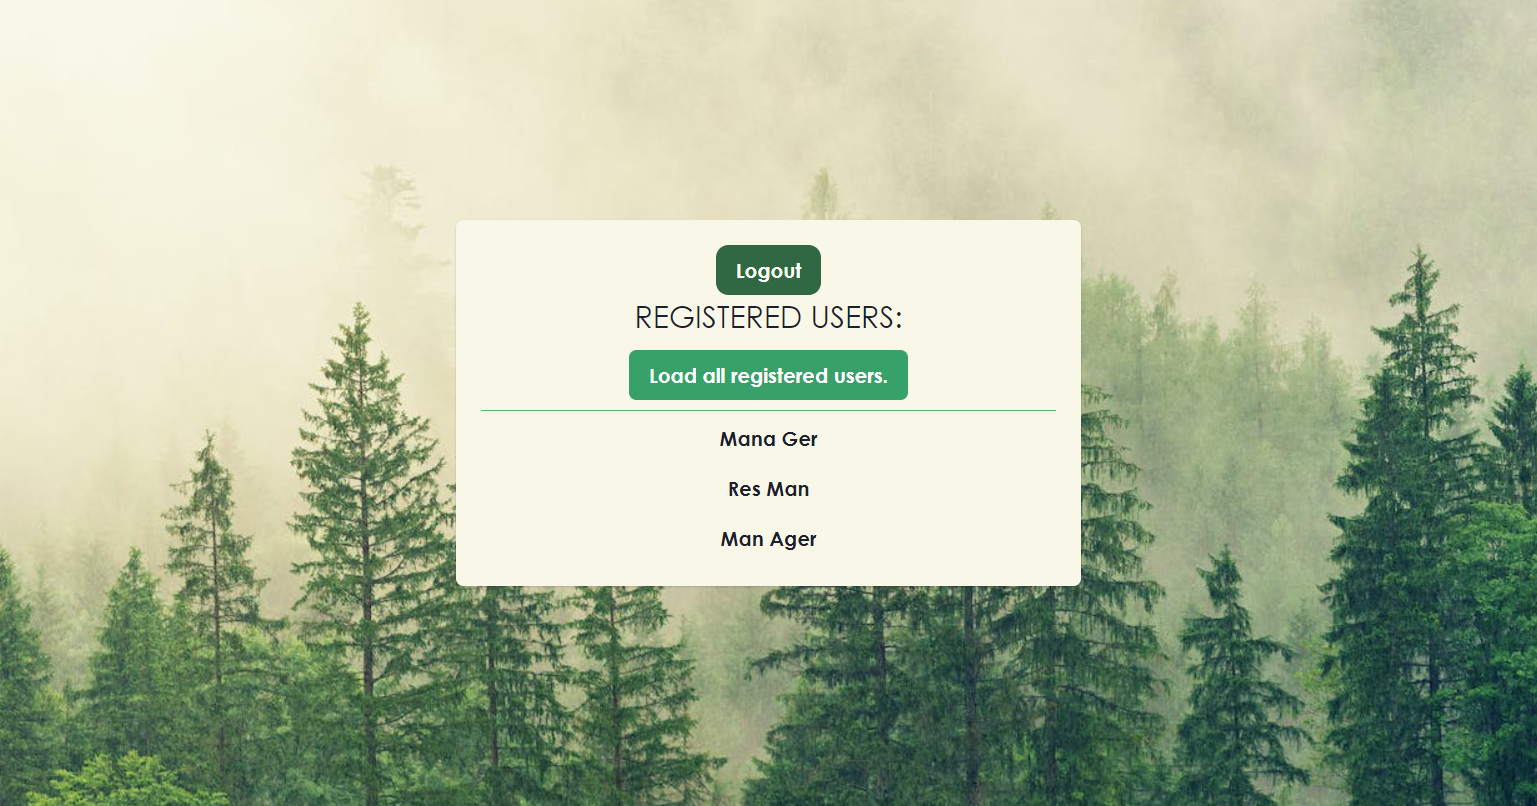
\includegraphics[scale=0.5]{slike/test3selres.PNG} %veličina slike u odnosu na originalnu datoteku i pozicija slike
	\centering
\end{figure}
\noindent Administrator može potvrditi korisnike i na kraju dobiva popis svih korisnika aplikacije. \\

\noindent \textbf{4. ispitni slučaj: Ispitivanje unosa broja tragača od strane istraživača}\\
U ovom ispitivanju testiramo zahtjev istraživača za brojem tragača. Istraživač može zatražiti broj tragača za određenu vrstu pretrage. Želimo vidjeti što se dogodi ako se unese samo jedan potreban tragač, a na ostala mjesta se upiše 0. Očekujemo da sustav pošalje zahtjev voditelju za jednim tragačem, a ostale vrijednosti ignorira. \\
\textbf{Test:}
\begin{figure}[H]
	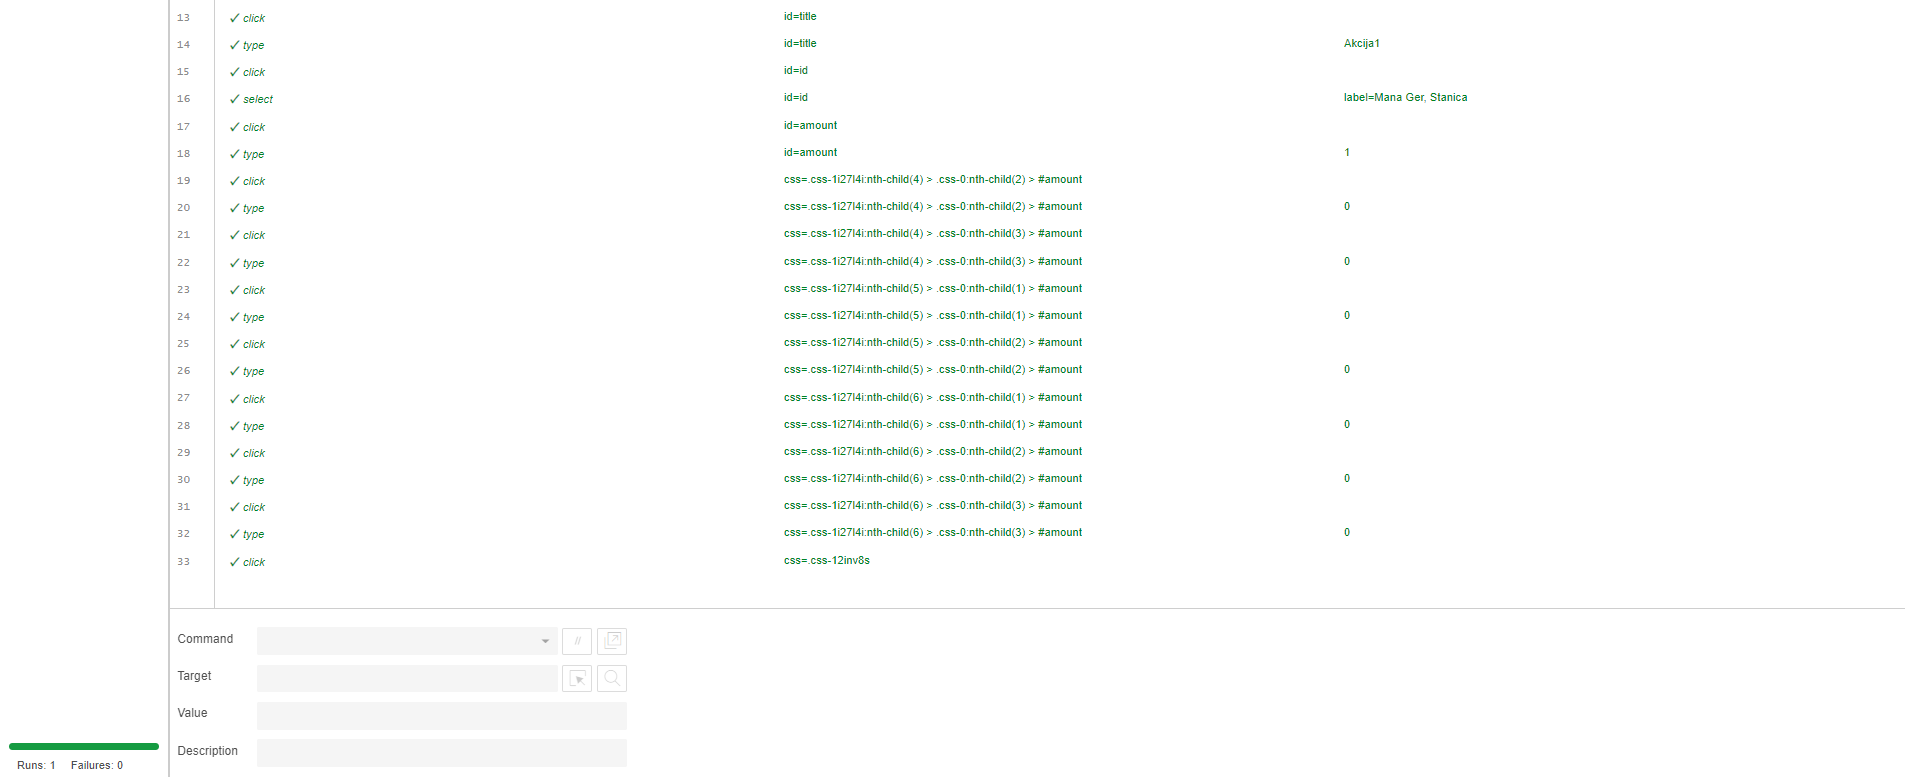
\includegraphics[scale=0.4]{slike/test4sel.PNG} %veličina slike u odnosu na originalnu datoteku i pozicija slike
	\centering
\end{figure}
\noindent \textbf{Rezultat:}
\begin{figure}[H]
	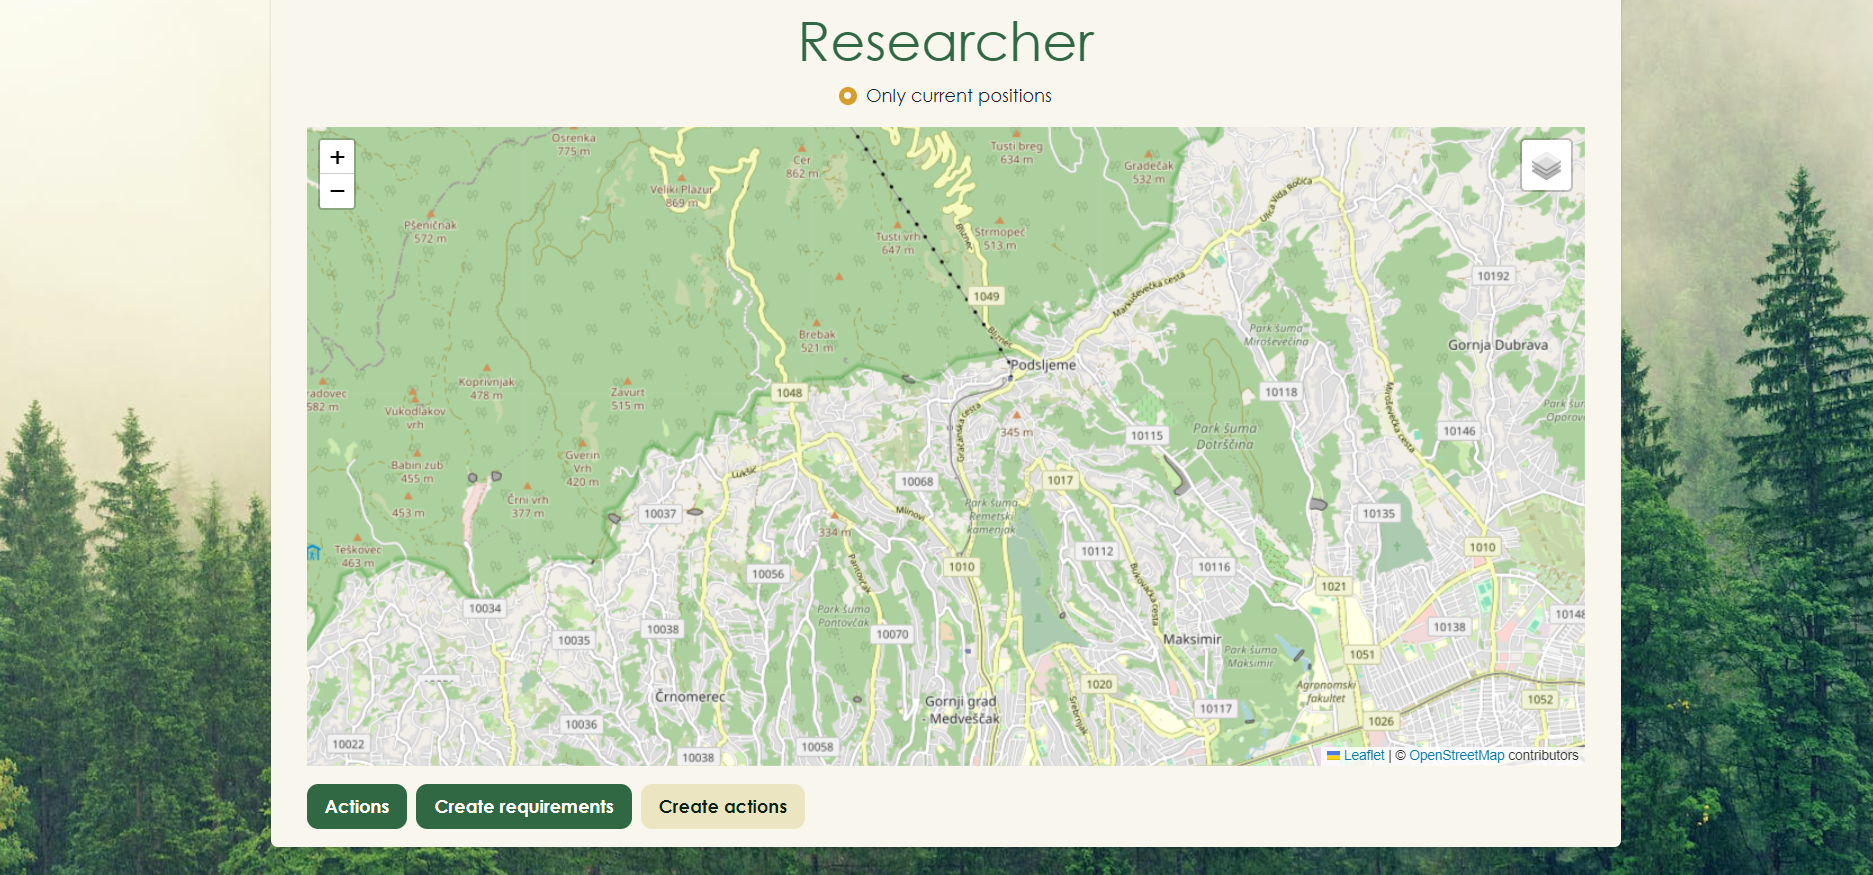
\includegraphics[scale=0.4]{slike/seltestres2copy.PNG} %veličina slike u odnosu na originalnu datoteku i pozicija slike
	\centering
\end{figure}
\noindent Istraživač uspješno šalje zahtjev za jednim tragačem i vraća se na početnu stranicu \\

\eject 


\section{Dijagram razmještaja}

\noindent Dijagram razmještaja je strukturni statički UML dijagram koji opisuje topologiju sustava i usredotočen je na odnos sklopovskih i programskih dijelova. Na korisničkom računalu nalazi se web preglednik. Na poslužiteljskom računalu nalazi se poslužitelj web aplikacije i poslužitelj baze podataka. Klijenti preko web preglednika pomoću HTTP veze komuniciraju s poslužiteljem web aplikacije.

\begin{figure}[H]
	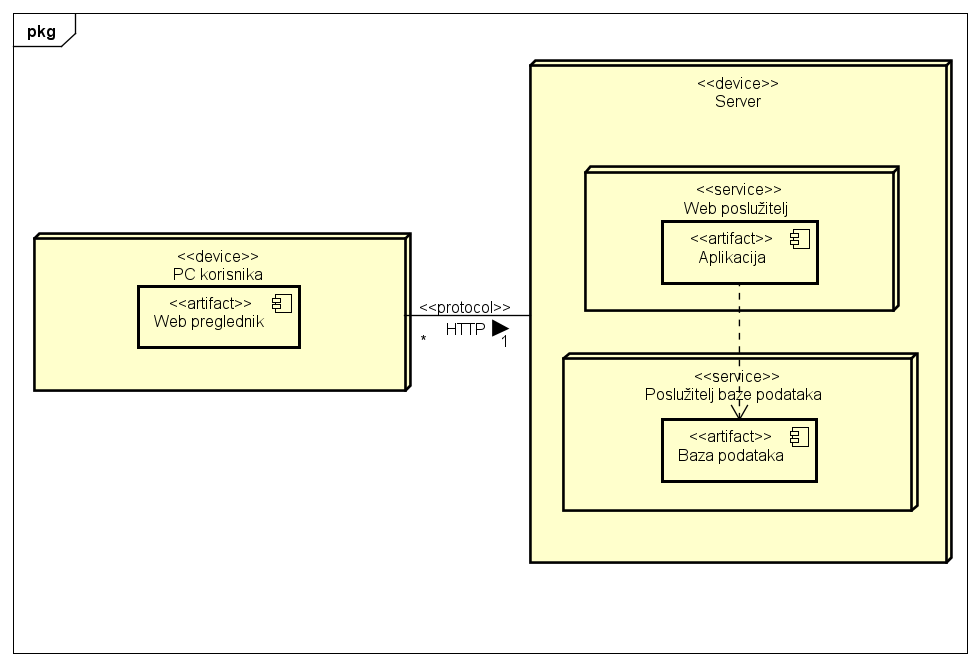
\includegraphics[scale=0.5]{slike/dijagram_razmjestaja.PNG} %veličina slike u odnosu na originalnu datoteku i pozicija slike
	\centering
\end{figure}

\eject 

\section{Upute za puštanje u pogon}

\textbf{\textit{dio 2. revizije}}\\

\textit{U ovom poglavlju potrebno je dati upute za puštanje u pogon (engl. deployment) ostvarene aplikacije. Na primjer, za web aplikacije, opisati postupak kojim se od izvornog kôda dolazi do potpuno postavljene baze podataka i poslužitelja koji odgovara na upite korisnika. Za mobilnu aplikaciju, postupak kojim se aplikacija izgradi, te postavi na neku od trgovina. Za stolnu (engl. desktop) aplikaciju, postupak kojim se aplikacija instalira na računalo. Ukoliko mobilne i stolne aplikacije komuniciraju s poslužiteljem i/ili bazom podataka, opisati i postupak njihovog postavljanja. Pri izradi uputa preporučuje se \textbf{naglasiti korake instalacije uporabom natuknica} te koristiti što je više moguće \textbf{slike ekrana} (engl. screenshots) kako bi upute bile jasne i jednostavne za slijediti.}


\textit{Dovršenu aplikaciju potrebno je pokrenuti na javno dostupnom poslužitelju. Studentima se preporuča korištenje neke od sljedećih besplatnih usluga: \href{https://aws.amazon.com/}{Amazon AWS}, \href{https://azure.microsoft.com/en-us/}{Microsoft Azure} ili \href{https://www.heroku.com/}{Heroku}. Mobilne aplikacije trebaju biti objavljene na F-Droid, Google Play ili Amazon App trgovini.}


\eject 